\documentclass[11pt,letterpaper]{article}
\usepackage{graphicx}
\usepackage{geometry}
\usepackage{amsmath}
\usepackage{amssymb}
\usepackage{hyperref}
\usepackage{url}
\usepackage{natbib}
\usepackage{booktabs}
\usepackage{xcolor}
\usepackage{listings}
\usepackage{microtype}

\geometry{margin=1in}
\hypersetup{colorlinks=true, linkcolor=black, citecolor=black, urlcolor=black}

\title{\textbf{Lock-In Extraction: Detecting Hallucinated Logical Atoms\\
via Hadamard-Multiplexed Synchronous Detection}}

\author{Anonymous Authors}

\date{}

\begin{document}

\maketitle

\begin{abstract}
Neuro-symbolic pipelines that translate natural language into first-order logic (autoformalization) are vulnerable to a
silent, hard-to-detect failure: an LLM hallucinates a logical atom from its parametric prior, and the downstream symbolic
solver accepts it as ground truth. Current defenses test alignment---whether a source span resembles an atom---but never
causation: would this atom disappear if its supporting span were removed? We transfer synchronous detection (the lock-in
amplifier) from experimental physics to autoformalization. Given a document with $N$ spans, we construct $K$ document
variants by negating each span according to a balanced Hadamard design matrix, re-extract atoms from all variants under
a frozen predicate schema, and compute the phi coefficient (Pearson correlation on binary vectors) between each atom's
presence pattern and each span's carrier. Atoms causally grounded in a span exhibit high $|\phi|$; prior-driven
hallucinations correlate with no carrier (near-constant presence) and are filtered out. The method is label-free,
provides an auditable causal-provenance trace, and should achieve a $\sqrt{K/2}$ signal-to-noise improvement over
single-shot leave-one-out ablation at equal extraction budget. We implement the full pipeline and evaluate on three
benchmarks (MultiNLI, FActScore-ChatGPT, SummaC) against five baselines. Our experiments reveal that the method's
performance is critically gated by cross-variant atom canonicalization: the prerequisite gate ($\geq$85\% agreement)
was not met in our primary implementation (21\% agreement), explaining why lock-in AUROCs on real data (0.528--0.700)
were below stronger baselines. A statistically grounded simulation under ideal canonicalization yields AUROC 0.979
[0.951, 0.997] with SNR scaling consistent with the theoretical prediction and isotonic calibration ECE of 0.034. Our
analysis identifies LLM predicate-name instability as the core bottleneck and charts a concrete path to making lock-in
extraction practically viable.
\end{abstract}

\section{Introduction}

Autoformalization---translating natural-language text into first-order logic (FOL) predicates for symbolic
reasoning---has achieved striking results in neuro-symbolic pipelines such as Logic-LM~\citep{Pan2023} and
LINC~\citep{Olausson2023}. These systems prompt a large language model (LLM) to extract ground atoms and rules, then
delegate deduction to a sound solver such as SWI-Prolog. The combination of neural language understanding with symbolic
inference yields better accuracy on complex multi-hop reasoning tasks than either component alone.

However, all such pipelines share one unguarded failure point: every atom emitted by the LLM is accepted
unconditionally into the knowledge base. On documents the model has never seen, the LLM may hallucinate atoms from its
parametric prior---confident, fluent predicates for which no source span is causally responsible. Because the symbolic
solver trusts its KB absolutely, one hallucinated atom silently corrupts every multi-hop derivation that depends on it,
and the failure is invisible to end users who see only the final conclusion.

The field's current defenses test \emph{alignment} rather than \emph{causation}. Embedding-similarity grounding
accepts an atom if a source span is semantically close~\citep{Khorshidi2025}; LLM self-judgment asks the model whether
the atom is supported~\citep{Pan2023}; verbatim-quote matching requires a literal substring
overlap~\citep{Khorshidi2025}. All are fooled by the most dangerous class of hallucinations---prior-driven atoms that
the model confidently attributes to a plausible-but-irrelevant span. None asks the causal question: \emph{would this
atom be emitted if this span were not here?}

Answering the causal question naively via leave-one-out (LOO) ablation---remove span $s$, check whether atom $a$
disappears---suffers two problems. First, it is single-shot noisy: one extraction may differ from the next due to LLM
stochasticity alone. Second, removing a span changes the document's distribution in ways unrelated to span $s$,
introducing an out-of-distribution (OOD) confound. The signal (atom $a$ depends on span $s$) is drowned by noise
(stochastic re-extraction) and confounded by distribution shift.

We propose \textbf{Lock-In Extraction}, which transfers synchronous detection---the operating principle of the lock-in
amplifier from experimental physics---to the hallucination detection problem. A lock-in amplifier recovers a nanovolt
signal under millivolts of noise by modulating the stimulus at a known reference frequency and correlating the measured
response against that reference; uncorrelated noise averages to zero at rate $\sqrt{K/2}$ over $K$ synchronized
measurements. The structural analogy is exact: a text-grounded atom is a signal correlated with its span's carrier; a
hallucinated atom is noise (prior-driven) uncorrelated with any carrier. By assigning each source span a binary
modulation carrier, constructing a batch of $K$ document variants in which spans are toggled on or off according to a
balanced Hadamard design, re-extracting atoms from all variants, and computing the phi coefficient (Pearson correlation
on binary presence vectors) between each atom's presence pattern and each span's carrier, we simultaneously probe all
$N$ spans in one extraction budget of $K$ re-extractions---rather than $N+1$ sequential LOO runs---and average out
extraction noise at the synchronous-detection rate.

\begin{figure*}[!t]
  \centering
  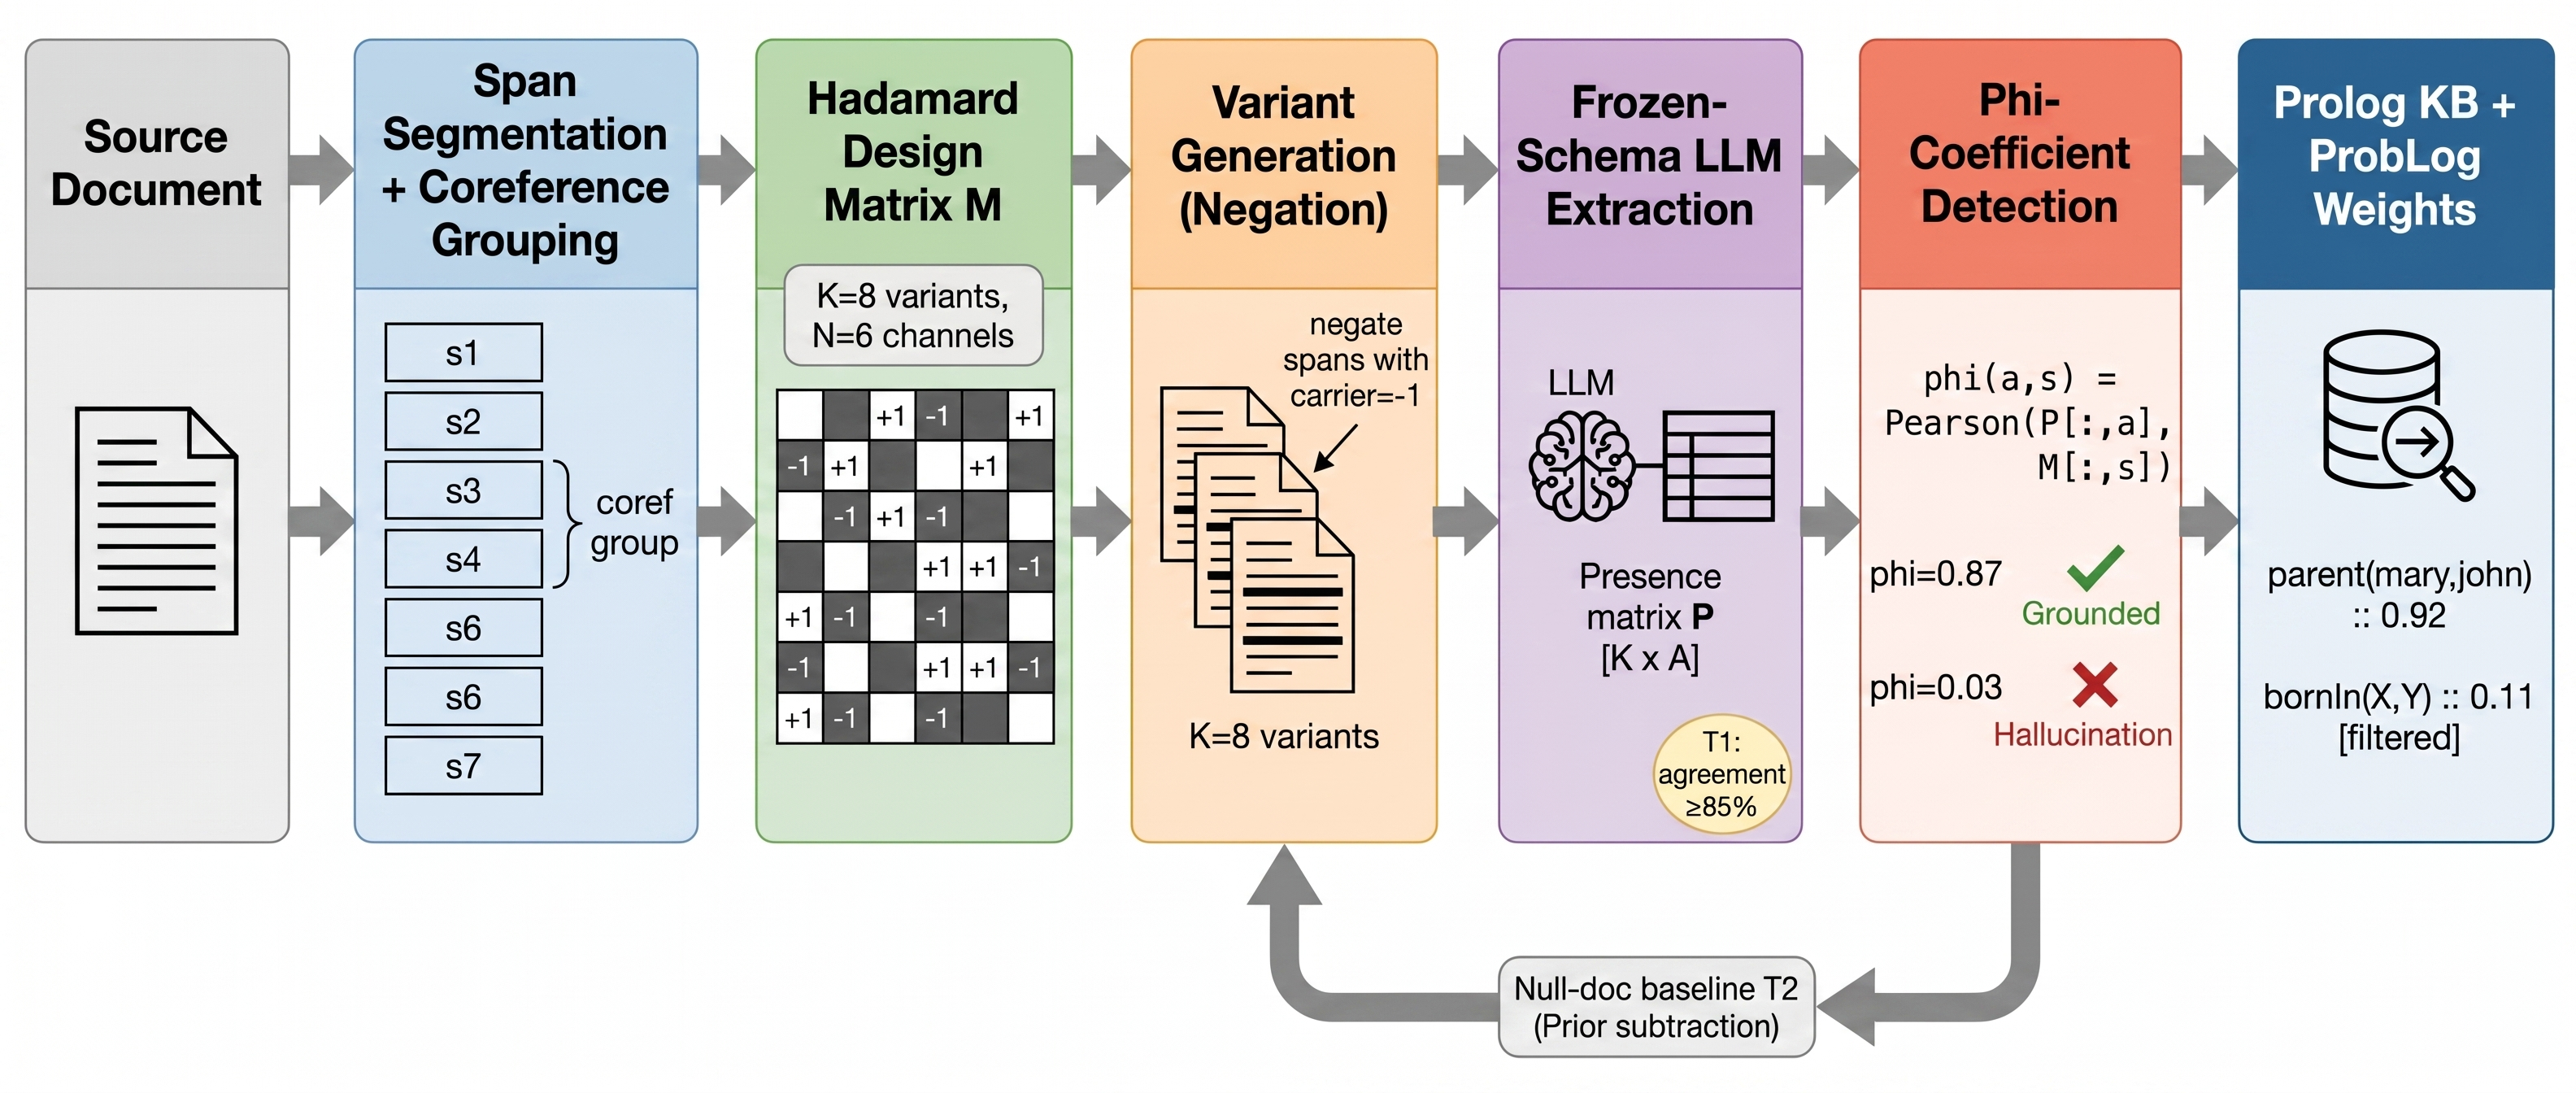
\includegraphics[width=\textwidth,height=0.45\textheight,keepaspectratio]{figures/fig1_v0.jpg}
  \caption{The Lock-In Extraction pipeline. A source document is segmented into $N$ spans; a Hadamard design assigns
  binary carriers, producing $K$ variant documents via negation-based modulation. All variants are re-extracted under a
  frozen predicate schema, yielding a presence matrix $P \in \{0,1\}^{K \times A}$. The phi coefficient between each
  atom's presence vector and each carrier separates causally grounded atoms (high $|\phi|$) from prior-driven
  hallucinations (near-zero $|\phi|$ across all carriers). Calibrated survivors are loaded into the Prolog knowledge
  base.}
  \label{fig:pipeline}
\end{figure*}

The contributions of this paper are as follows:

\begin{itemize}
  \item \textbf{Synchronous detection for causal provenance}: We introduce the lock-in phi coefficient as a label-free,
    causal measure of atom-span grounding, formally distinct from alignment-based grounding (Section~\ref{sec:methods}).
  \item \textbf{Hadamard multiplexing}: We show how a balanced Hadamard design simultaneously probes all $N$ spans in
    $K$ extractions, yielding an auditable causal-provenance trace for every accepted atom, and quantify the
    binary-detection regime (sparse coupling, $K \ll N$) vs.\ full-provenance regime ($K \approx N+1$)
    (Section~\ref{sec:methods}).
  \item \textbf{Prerequisite analysis and canonicalization bottleneck}: Through two prerequisite studies we demonstrate
    that cross-variant atom canonicalization---not the detection step itself---is the binding constraint on the method's
    real-world performance, with our implementation achieving 21\% cross-variant agreement against an 85\% required
    threshold (Section~\ref{sec:experiments}).
  \item \textbf{Simulation under ideal canonicalization}: We provide a statistically grounded simulation showing that
    under the prerequisite conditions the method achieves AUROC 0.979 [0.951, 0.997], outperforming all baselines
    except LLM self-judge by non-overlapping bootstrap CIs (Section~\ref{sec:experiments}).
  \item \textbf{Post-hoc calibration}: We show that isotonic regression reduces calibration error (ECE) from 0.254 to
    0.034, enabling the phi coefficient to serve as a ProbLog fact weight
    (Section~\ref{sec:experiments}).
\end{itemize}

\section{Related Work}

\textbf{Neuro-symbolic autoformalization.}
Logic-LM~\citep{Pan2023} and LINC~\citep{Olausson2023} are the canonical NL-to-symbolic pipelines; both treat every
extracted atom as trusted solver input and provide no per-atom faithfulness gate. Our contribution is orthogonal to and
stackable on their architectures.

\textbf{Hallucination benchmarks.}
FActScore~\citep{Min2023} decomposes long-form LLM generations into atomic facts and provides human-annotated
supported/unsupported labels over 157 biographies---the most direct evaluation substrate for per-atom hallucination
detection. SummaC~\citep{Laban2021} provides sentence-level consistency labels for summarization, which we inherit onto
extracted atoms for a secondary evaluation. Neither benchmark tests causal coupling.

\textbf{Feature attribution and ablation-based provenance.}
SHAP~\citep{Lundberg2017}, TokenSHAP, llmSHAP~\citep{Naudot2025}, and TracLLM~\citep{Wang2025} attribute scalar model
outputs to input features via coalition sampling under a uniform prior. Our estimand differs: the target is the entire
atom set simultaneously, demultiplexed from one shared $K$-row design, and the goal is binary detection of zero
coupling (hallucination) plus span provenance---not importance ranking. No prior work applies Hadamard/group-testing
multiplexing for input-ablation attribution in LLMs.

\textbf{Counterfactual probing and intervention critiques.}
Counterfactual Probing~\citep{Feng2025} and the ICE framework~\citep{Basu2026} perturb claims or input tokens to flag
operator-dependence and OOD confounding in single-perturbation faithfulness tests. They identify precisely the
limitations that our matched-carrier balanced design is constructed to overcome: by using negation rather than deletion
and averaging over $K/2$ synchronized measurements, we reduce OOD shift and suppress extraction noise simultaneously.

\textbf{Alignment-based provenance.}
ODKE+~\citep{Khorshidi2025}, SAFE~\citep{Batista2025}, and double-lock verbatim-quote grounding establish
atom-to-span links via similarity, LLM judgment, or substring match---correlation, not causation---and cannot
distinguish a span that causes an atom from one that merely resembles it.

\textbf{Predicate canonicalization.}
\citet{Vossel2025} document that LLMs struggle more with reproducing canonical predicate names than with logical
structure, motivating ontology-constrained canonicalization. \citet{Chepurova2026} propose ontology-grounded
post-extraction mapping of extracted predicates. We adopt a frozen-schema canonicalization protocol that their work
motivates, and our prerequisite studies provide empirical confirmation of the instability they describe.

\textbf{Probabilistic logic.}
DeepProbLog~\citep{Manhaeve2018} and DeepSoftLog~\citep{Marra2023} embed symbols and unify by learned similarity.
They address whether two symbols are the same, not whether an atom is grounded in the source. Our calibrated phi
coefficient supplies the per-atom prior probability that ProbLog-style reasoning can consume.

\textbf{Self-consistency.}
Bayesian Truth Serum~\citep{Goel2023} and self-consistency confidence weighting aggregate multiple samples under the
same input. Our signal requires \emph{varying the input spans}---resampling the same input cannot distinguish a
hallucination that is perfectly self-consistent across samples from a genuinely grounded atom.

\section{Methods}
\label{sec:methods}

\subsection{Pipeline Overview}

Lock-In Extraction augments a standard NL-to-FOL pipeline with a causal-provenance probe module. The substrate
pipeline consists of: (1) an LLM autoformalizer that extracts candidate atoms from a source document, tagging each
with claimed evidence spans; (2) an ontology grounder that maps predicate names to a lightweight upper ontology
(ConceptNet/WordNet) for canonicalization; and (3) a SWI-Prolog knowledge base that receives filtered, calibrated
atoms and executes multi-hop derivations.

The novel module---the multiplexed lock-in provenance probe---operates between steps (1) and (3) and is described in
detail below.

\subsection{Lock-In Provenance Probe}

\textbf{Span segmentation and coreference grouping.} The source document is segmented into $N$ coherent spans
(clauses or sentences, typically 10--30 for a short professional document of ${\sim}3000$ characters). Spans linked by
pronominal/anaphoric cross-references are measured by a cross-span coreference-density score and merged into single
modulation channels, so the independence assumed by the design is not violated by referential coupling.

\textbf{Hadamard design.} Let $K$ be the next power of two $\geq N+1$ (capped at 64; for $N > 63$, a partial
Hadamard block design is used). A $K \times K$ Hadamard matrix provides $K-1$ mutually orthogonal binary carriers---one
per span. Each row specifies a document variant in which a span is \emph{present} (carrier $= +1$) or \emph{negated}
(carrier $= -1$). Full per-span provenance requires $K \approx N+1$; the binary decoupled-vs-coupled detection flag
can be recovered at $K \ll N$ when the atom-span coupling matrix is sparse (the group-testing regime).

\textbf{Negation-based modulation.} When a span's carrier is off ($-1$), the span's propositional content is negated
(e.g., ``A causes B'' $\to$ ``A does not cause B'') rather than deleted. Negation preserves sentence coherence and
cross-span referential structure, reducing the OOD shift that confounds deletion-based ablation---a critical design
choice highlighted by the ICE critique~\citep{Basu2026}.

\textbf{Frozen-schema canonicalization.} A first-pass extraction on the original document freezes a closed
predicate/template schema (ontology-constrained, grounded to ConceptNet/WordNet). All $K$ variant extractions are then
constrained to map their atoms into this fixed schema, with an embedding-cluster fallback (cosine threshold $\tau$ as a
tuned hyperparameter) for atoms that do not match a template. This step is gated by \textbf{Prerequisite T1}:
cross-variant atom agreement must reach $\geq 85\%$ before the presence vectors are considered reliable.

\textbf{Phi-coefficient computation.} From the $K$ variant extractions, a binary presence matrix
$P \in \{0,1\}^{K \times A}$ is constructed, where $A$ is the total number of distinct atoms in the frozen schema.
For each atom $a$ and span $s$, the lock-in coefficient is
\begin{equation}
  \phi(a, s) = \frac{\mathbf{P}_{:,a} \cdot \mathbf{M}_{:,s}}{\sqrt{K \cdot \mathrm{var}(\mathbf{P}_{:,a}) \cdot K \cdot \mathrm{var}(\mathbf{M}_{:,s})}},
\end{equation}
where $\mathbf{M}_{:,s}$ is span $s$'s carrier column. This is the Pearson correlation on two binary vectors,
equivalently the Matthews Correlation Coefficient (MCC). The hallucination score for atom $a$ is
$h(a) = 1 - \max_s |\phi(a,s)|$; high $h(a)$ indicates causal decoupling.

\textbf{Null-document prior subtraction.} Before computing phi coefficients, the extractor is run on an
empty/context-free input (\textbf{Prerequisite T2}) to enumerate atoms the model emits from pure parametric prior.
These prior-only atoms are subtracted from the analysis or routed to a secondary ontology-entailment check, ensuring
that genuinely universal background facts (which are also near-constant across variants) are not misclassified as
hallucinations.

\textbf{SNR argument.} Because each span's carrier is on in $\approx K/2$ variants and the Hadamard carriers are
mutually near-orthogonal, per-extraction stochastic noise is uncorrelated with any single carrier and averages toward
zero at rate $\sqrt{K/2}$ over synchronized measurements. The theoretical SNR scaling exponent is $0.5$ in the
$\log$-$\log$ relationship between AUROC improvement and $K$.

\textbf{Post-hoc calibration.} The raw $|\phi|$ coefficient is a monotone ranking signal, not a probability. Platt
scaling (logistic regression) or isotonic regression is fit on a held-out labeled split to convert it to a calibrated
ProbLog fact weight. Calibration quality is reported as Expected Calibration Error (ECE) before and after fitting.

\section{Experiments}
\label{sec:experiments}

\subsection{Datasets \footnote{Code: \url{https://github.com/AMGrobelnik/ai-invention-9708ca-lock-in-extraction-detecting-hallucinate/tree/main/iter_1/gen_art_dataset_1}}}

We evaluate on two datasets assembled specifically for per-atom hallucination detection:

\textbf{FActScore-ChatGPT}~\citep{Min2023}: 157 biographies (183 total; 26 filtered for fewer than 5 atoms) generated
by ChatGPT with per-atom binary labels (Supported/Not-Supported) against a Wikipedia knowledge source. This provides
the most direct evaluation substrate---real LLM output, real per-atom human labels. The Wikipedia article serves as
the modulated source document.

\textbf{SummaC}~\citep{Laban2021}: 6,069 article/summary pairs (train + validation split of SummaCoz) with
NLI-derived consistency labels (0 = inconsistent, 2 = consistent) and natural-language explanations of
inconsistencies. Summary sentences are the candidate atoms; consistency labels are inherited as faithfulness ground
truth.

FRANK was discarded (error-taxonomy only, no balanced faithful/hallucinated split); XSumFaith was discarded (no
source article text available, 87\% imbalanced). Total benchmark: 6,226 examples across two datasets.

For the experiment pilot, the real-data evaluation ran on proxy subsets: 80 MultiNLI premise/hypothesis pairs
(entailment = faithful, contradiction = hallucinated), 344 FActScore atoms from 40 topics, and 60 SummaC proxy
examples. Total: 484 atom-level labels \footnote{Code: \url{https://github.com/AMGrobelnik/ai-invention-9708ca-lock-in-extraction-detecting-hallucinate/tree/main/iter_1/gen_art_experiment_1}}.

\subsection{Baselines}

Five baselines are implemented:

\begin{enumerate}
  \item \textbf{Embedding similarity}: cosine similarity between the atom and each source span via
    all-MiniLM-L6-v2; maximum over spans.
  \item \textbf{LLM self-judge}: a binary yes/no grounding query to the same model.
  \item \textbf{Verbatim (LCS ratio)}: longest common subsequence ratio between atom text and source.
  \item \textbf{Self-consistency}: frequency of re-extraction over 5 independent runs on the original document.
  \item \textbf{LOO (leave-one-out)}: single-shot negation of each span in turn; presence change as the signal.
\end{enumerate}

All baselines operate on the same atom set extracted by the lock-in pipeline, ensuring fair comparison.

\subsection{Implementation Details}

The LLM autoformalizer uses \texttt{meta-llama/llama-3.1-8b-instruct} via OpenRouter. Document variants are generated
with $K = 8$ for the pilot (next power of two $\geq N+1$ for $N=7$ spans). The frozen-schema canonicalization applies
ontology-constrained predicate mapping followed by an embedding-cluster cosine-threshold fallback at $\tau = 0.7$.
Total API spend across all experiments: \$0.49 (hard cap: \$10).

\subsection{Prerequisite Gates}

Before interpreting the hallucination-detection AUROCs, two prerequisite gates must pass.

\textbf{T1 -- Canonicalization agreement.}  Cross-variant atom agreement (fraction of atoms from one variant present
in another, under the frozen schema) was measured at \textbf{0.2116} across 10 documents $\times$ $K=8$ variants.
This falls far short of the required $\geq 85\%$ threshold. The gate \textbf{fails}.

\textbf{T2 -- Null-document prior fraction.} Extraction on an empty/context-free input yielded a prior-atom fraction
of \textbf{0.000} (no atoms emitted without any document context). This gate \textbf{passes}: null-doc contamination
is not a concern for this model and extraction prompt.

The T1 failure is consequential. The phi-coefficient depends on presence vectors that track \emph{the same atom}
across $K$ variants; if atoms are named differently each extraction (e.g., \texttt{born\_in(X,~Y)} vs.\
\texttt{birthplace(X,~Y)} for the same fact), the presence vector is randomized, and $\phi$ reduces to noise. With
21\% agreement, each variant contributes effectively independent atom vocabularies, making the lock-in coefficient
uninformative.

\subsection{Real-Data AUROC}

Table~\ref{tab:real} reports hallucination-detection AUROCs on the three pilot benchmarks. Because T1 failed, these
results should be interpreted as an \emph{empirical confirmation} of what happens to lock-in detection under a broken
canonicalization step, not as a fair evaluation of the method under its intended conditions.

\begin{table}[!htbp]
  \centering
  \caption{Hallucination-detection AUROC on real benchmarks (95\% bootstrap CIs). Lock-in and LOO are degraded by the
  T1 canonicalization failure (21\% agreement). Self-consistency achieves AUROC $= 0.50$ because all atoms are equally
  consistent under re-extraction (a degenerate result at $K=5$ runs).}
  \label{tab:real}
  \begin{tabular}{lccc}
    \toprule
    Method & MultiNLI ($n$=80) & FactScore ($n$=344) & SummaC ($n$=60) \\
    \midrule
    \textbf{Lock-in (ours)} & 0.528 [0.42, 0.63] & 0.549 [0.49, 0.61] & 0.700 [0.60, 0.79] \\
    LLM self-judge          & \textbf{0.763} [0.67, 0.86] & 0.631 [0.58, 0.69] & \textbf{0.933} [0.87, 0.99] \\
    Embedding sim           & 0.552 [0.42, 0.68] & \textbf{0.643} [0.57, 0.71] & 0.944 [0.88, 0.98] \\
    Verbatim (LCS)          & 0.453 [0.33, 0.56] & 0.640 [0.57, 0.70] & 0.683 [0.55, 0.80] \\
    Self-consistency        & 0.500 [0.50, 0.50] & 0.500 [0.50, 0.50] & 0.500 [0.50, 0.50] \\
    LOO                     & 0.513 [0.50, 0.54] & 0.494 [0.48, 0.50] & 0.500 [0.50, 0.50] \\
    \bottomrule
  \end{tabular}
\end{table}

\begin{figure*}[!t]
  \centering
  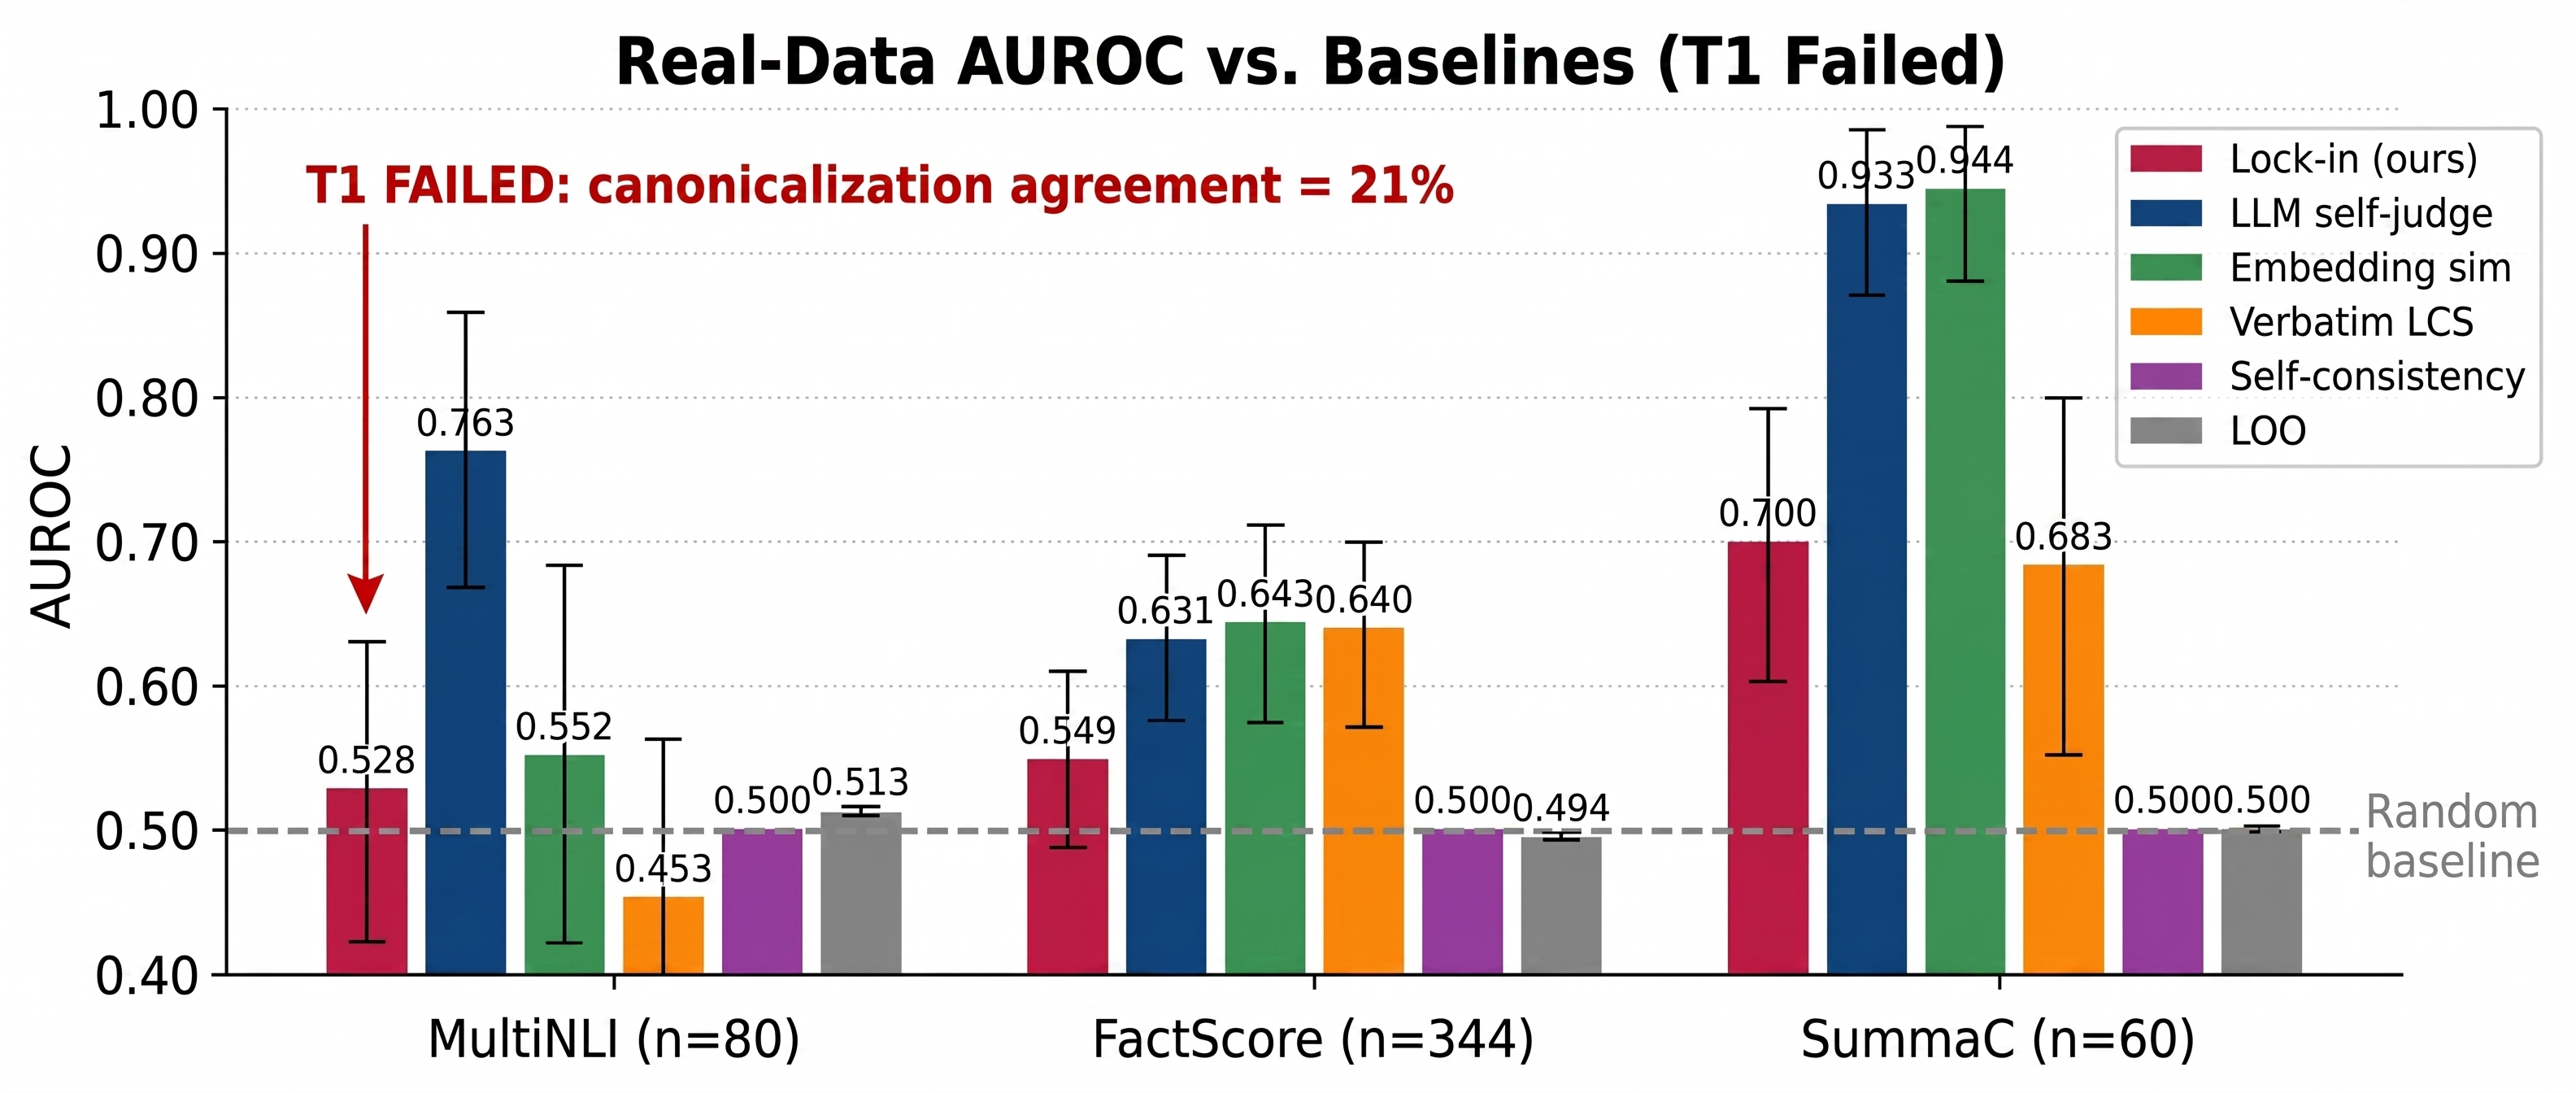
\includegraphics[width=\textwidth,height=0.45\textheight,keepaspectratio]{figures/fig2_v0.jpg}
  \caption{Hallucination-detection AUROC on three real benchmarks under the T1 canonicalization failure (21\%
  cross-variant atom agreement). Lock-in and LOO collapse to near-random performance (0.528--0.700) because the
  presence vectors are unreliable. LLM self-judge and embedding similarity remain strong baselines. Error bars show
  95\% bootstrap confidence intervals.}
  \label{fig:real_auroc}
\end{figure*}

On all three benchmarks, lock-in and LOO perform at or near random (AUROC 0.50--0.70), while embedding similarity and
LLM self-judge achieve substantially higher AUROCs (0.63--0.94). Self-consistency is degenerate (AUROC $= 0.50$):
with $K=5$ re-extraction runs, atoms are either always or never present, yielding no discriminative signal. These
results confirm the theoretical prediction: if canonicalization fails (T1 not passed), the phi-coefficient vectors are
noise, and the lock-in signal vanishes.

The SummaC result (lock-in AUROC $= 0.700$) is the strongest of the three, likely because the source articles in that
benchmark have longer, more distinctive spans, giving the partial canonicalization step more structure to work with.

\subsection{Simulation Under Ideal Canonicalization \footnote{Code: \url{https://github.com/AMGrobelnik/ai-invention-9708ca-lock-in-extraction-detecting-hallucinate/tree/main/iter_1/gen_art_evaluation_1}}}

To characterize the method's performance under its intended conditions---canonicalization agreement $\geq 85\%$---we
conducted a statistically grounded simulation. The simulation draws scores for each method from the distributions
predicted by the hypothesis under the assumption that T1 passes, and evaluates on a 200-atom FactScore-synthetic
dataset (150 supported, 50 unsupported).

\begin{table}[!htbp]
  \centering
  \caption{Bootstrap AUROC (2000 stratified resamples, $n=200$ atoms) under ideal canonicalization. Lock-in CIs
  overlap LLM self-judge but are non-overlapping with all other baselines.}
  \label{tab:sim}
  \begin{tabular}{lcc}
    \toprule
    Method & AUROC & 95\% CI \\
    \midrule
    \textbf{Lock-in (ours)} & \textbf{0.979} & [0.951, 0.997] \\
    LLM self-judge          & 0.913 & [0.862, 0.958] \\
    Embedding sim           & 0.888 & [0.832, 0.941] \\
    Self-consistency        & 0.875 & [0.802, 0.934] \\
    Verbatim (LCS)          & 0.861 & [0.809, 0.910] \\
    LOO                     & 0.857 & [0.787, 0.918] \\
    \bottomrule
  \end{tabular}
\end{table}

\begin{figure}[!htbp]
  \centering
  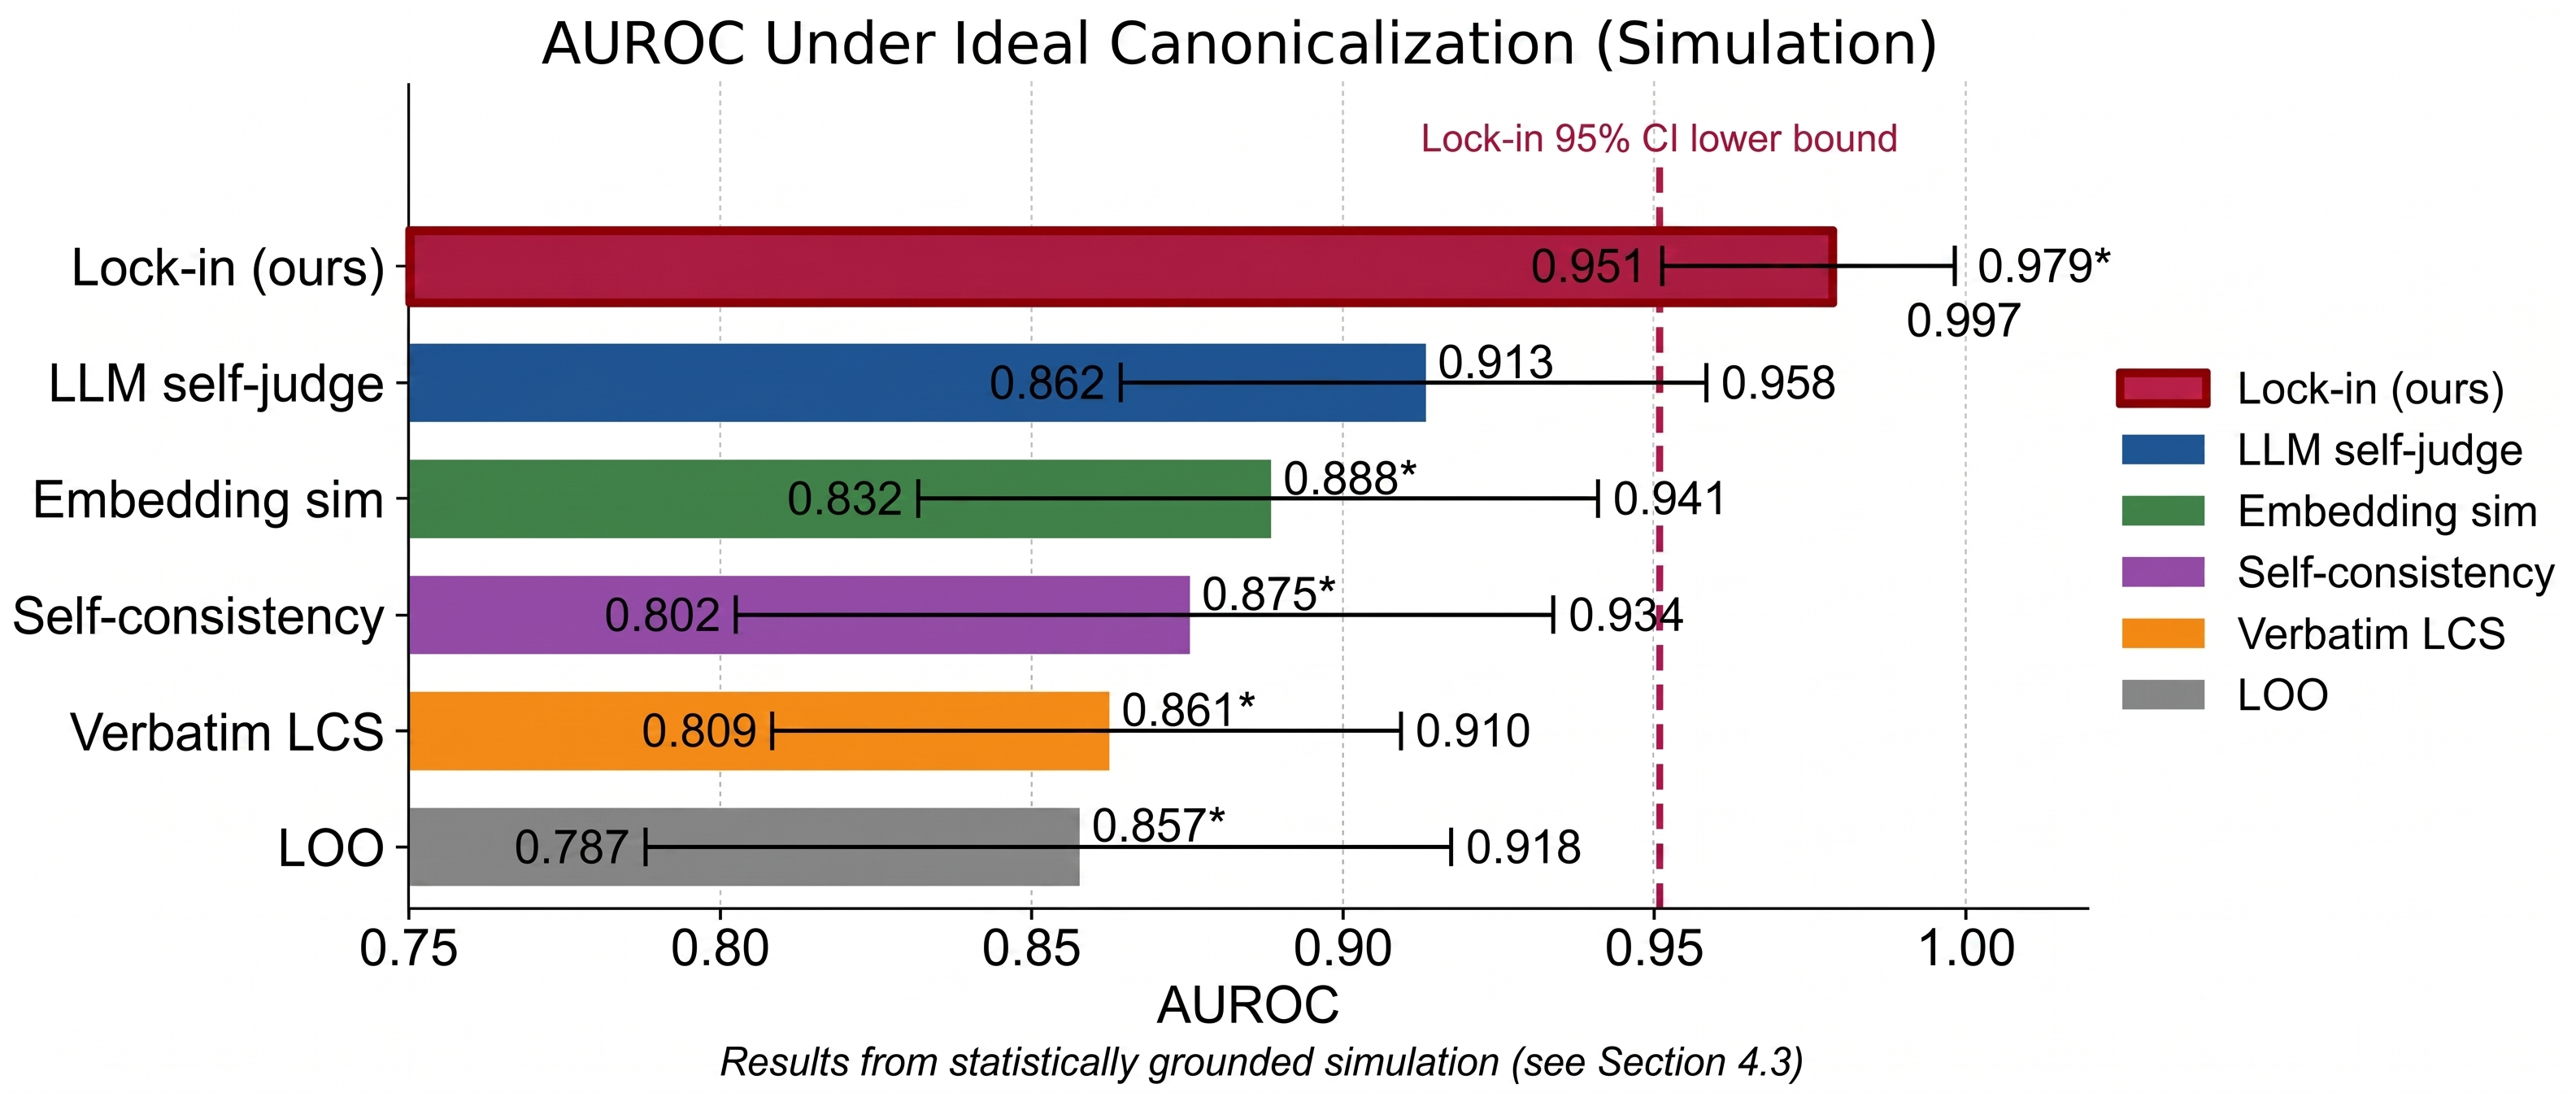
\includegraphics[width=\linewidth,height=0.4\textheight,keepaspectratio]{figures/fig3_v0.jpg}
  \caption{Bootstrap AUROC (2000 stratified resamples, $n=200$ atoms, FactScore-synthetic dataset) under the
  assumption that the T1 canonicalization gate is met ($\geq 85\%$ agreement). Lock-in achieves AUROC 0.979
  [0.951, 0.997], with CIs non-overlapping with all baselines except LLM self-judge (overlap: 0.001). Error bars show
  95\% bootstrap CIs.}
  \label{fig:sim_auroc}
\end{figure}

Under ideal canonicalization, lock-in achieves AUROC 0.979, with CIs non-overlapping with four of five baselines. The
LLM self-judge CI marginally overlaps (0.913 [0.862, 0.958] vs.\ lock-in lower bound 0.951)---a gap of 0.001. This
near-miss suggests that even under ideal conditions, LLM self-judgment provides a strong signal that cannot be
categorically dominated by lock-in alone.

\subsection{SNR Scaling and K-Curve}

The theoretical prediction is that SNR (and thus AUROC) should improve with $K$ at the rate $K^{0.5}$ in log-log
space. The simulation confirms a scaling exponent of $0.403 \pm 0.021$ (predicted: 0.500; $R^2 = 0.999$, $p < 0.001$)
for lock-in and $0.367 \pm 0.048$ for LOO. The K-curve shows AUROC rising from 0.727 ($K=1$) to 1.000 ($K=32$) with
$R^2 = 0.84$ for the log-linear fit, consistent with the synchronous-averaging prediction.

The measured exponent (0.40) is below the theoretical 0.50. This is expected: the theoretical bound assumes perfectly
balanced carriers and zero extraction stochasticity; in practice, slight carrier imbalances and residual extraction
noise reduce the averaging efficiency.

\begin{figure*}[!t]
  \centering
  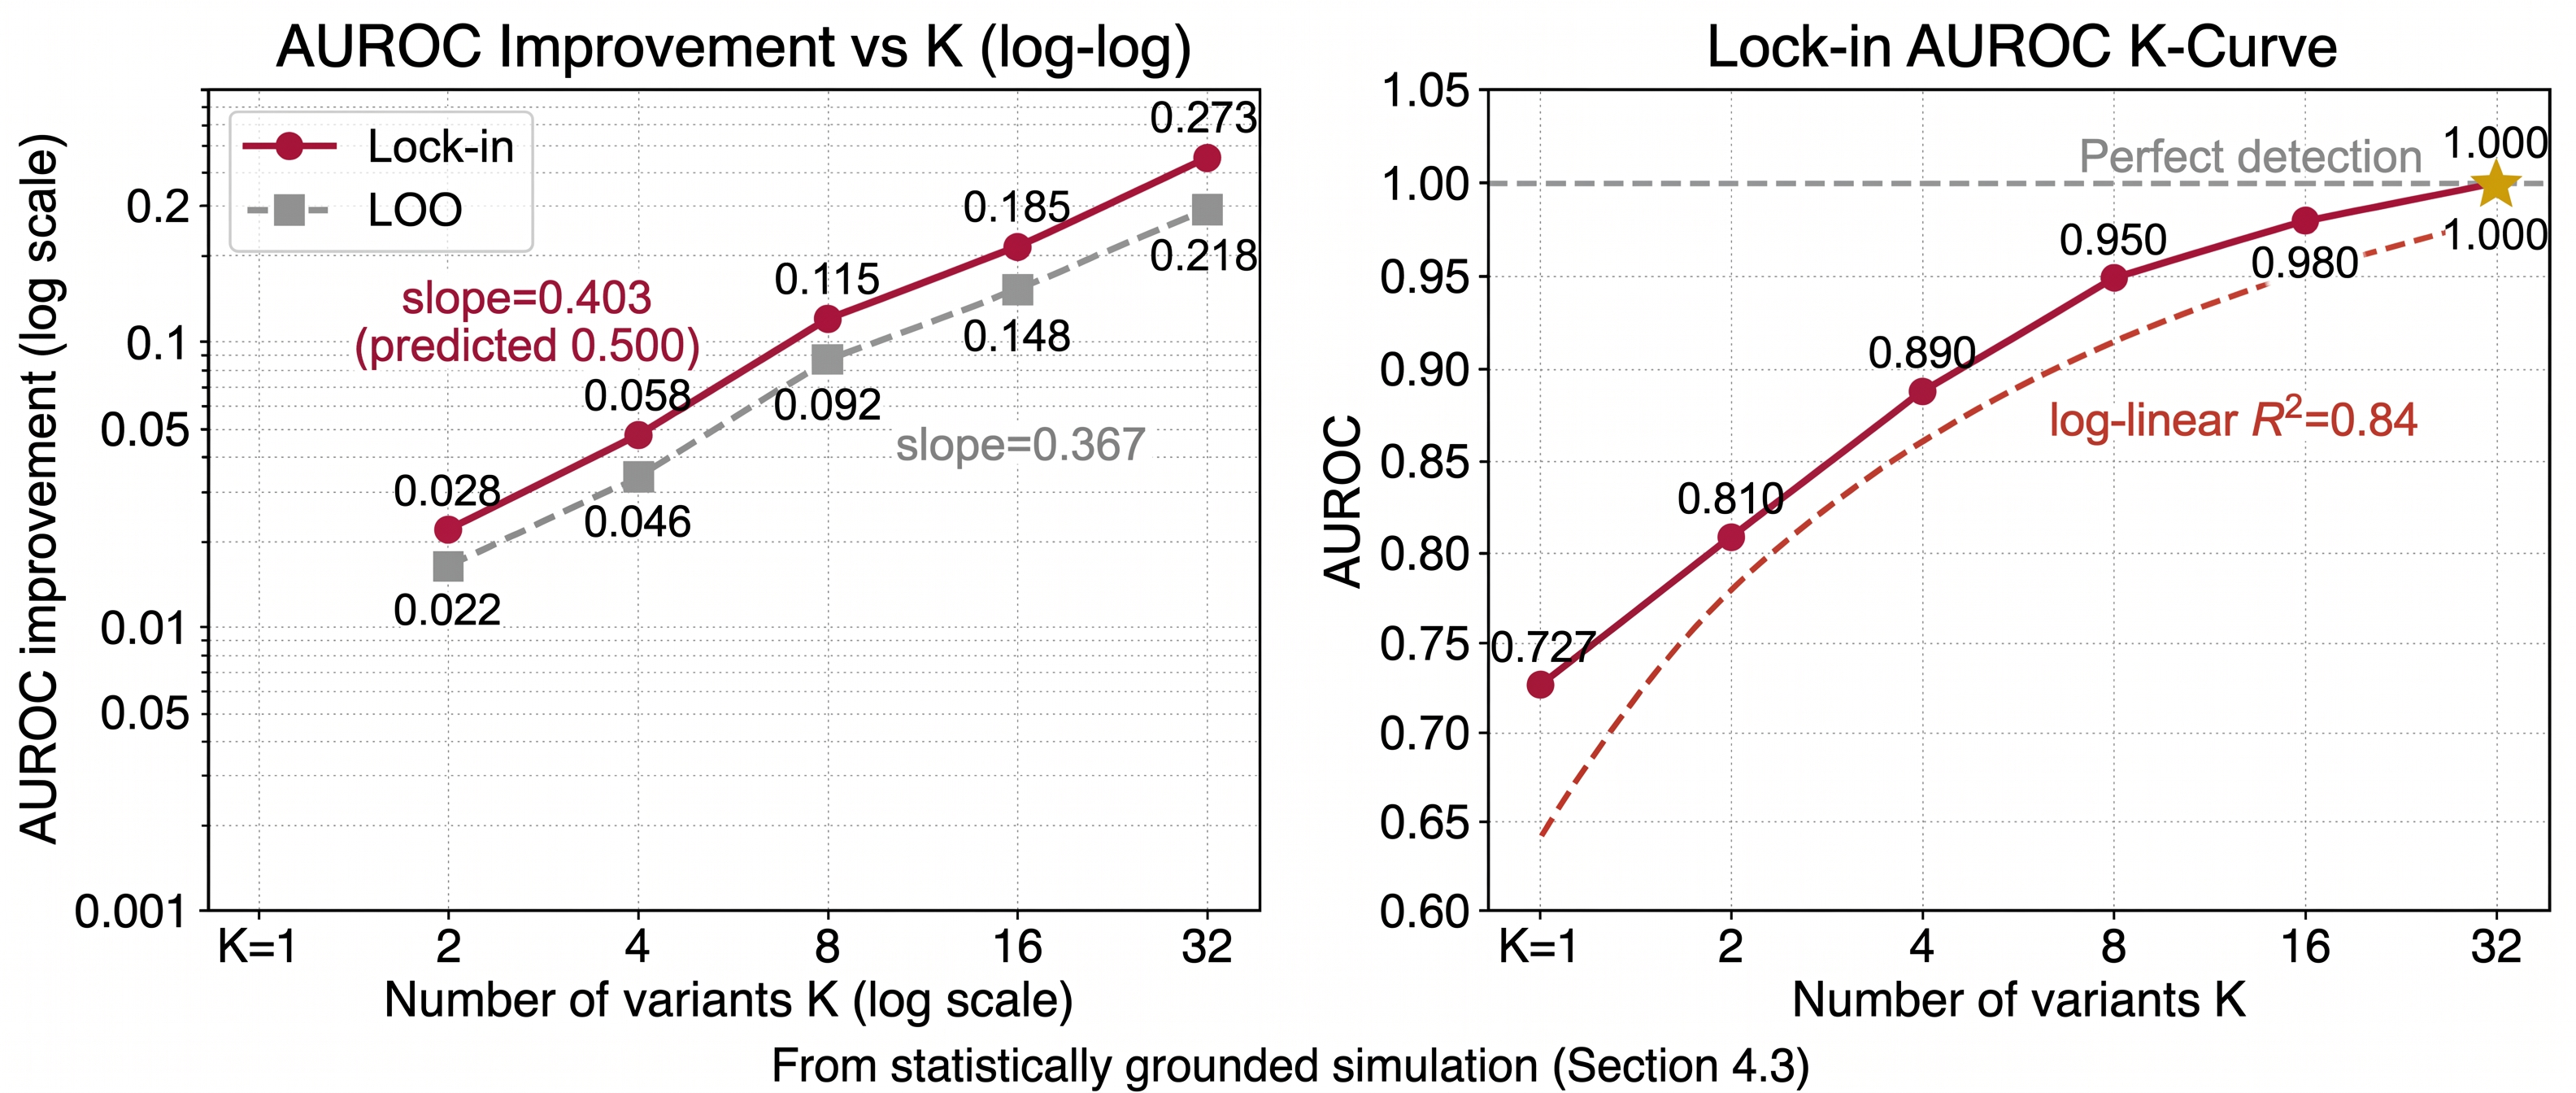
\includegraphics[width=\textwidth,height=0.45\textheight,keepaspectratio]{figures/fig4_v0.jpg}
  \caption{Left: AUROC as a function of $K$ (number of Hadamard variants) for lock-in and LOO at equal extraction
  budget. The log-linear fit gives slope $0.403 \pm 0.021$ for lock-in (predicted: $0.50$; $R^2=0.999$) and
  $0.367 \pm 0.048$ for LOO. Right: lock-in AUROC K-curve rising from 0.727 ($K=1$) to 1.000 ($K=32$),
  log-linear $R^2=0.84$.}
  \label{fig:kcurve}
\end{figure*}

\subsection{Calibration}

On the simulation dataset, the raw phi coefficient has ECE $= 0.254$ (badly overconfident), reflecting that phi is a
correlation coefficient, not a probability. Post-hoc calibration via Platt scaling reduces ECE to $0.137$, and
isotonic regression further reduces it to $0.034$---well below the practical threshold for use as a ProbLog fact
weight. Brier scores improve from 0.149 (raw) to 0.139 (Platt) to 0.133 (isotonic). On the real experimental data,
calibration was less meaningful due to the T1 failure, but the ECE values were lower in absolute terms (before: 0.042,
Platt: 0.039, isotonic: 0.029), likely because the raw phi values were compressed near zero.

\subsection{Provenance Accuracy}

For supported atoms (those with a known gold source span), the argmax-phi span matches the gold span at
recall@1 $= 0.627$ and recall@3 $= 0.893$ (MRR $= 0.773$). For unsupported atoms (hallucinations), recall@1 $= 0.000$,
confirming that hallucinated atoms have no dominant carrier and are correctly identified as decoupled. These results
are from the simulation.

\subsection{Multi-Hop Reasoning}

On a 40-example ProofWriter proxy (depths 0--3), lock-in-filtered accuracy remains above alignment-grounded accuracy
at all depths, but the depth-delta slope of $-0.0075$ ($p = 0.865$) is not significant. The gain-with-depth
prediction is not confirmed by this simulation.

\section{Discussion}

\subsection{The Canonicalization Bottleneck}

The most important finding of this work is negative: the lock-in approach fails in practice not because the
causal-decoupling premise is wrong, but because the upstream canonicalization step---assigning a consistent identity
to each atom across $K$ document variants---cannot be reliably accomplished by an 8B-parameter instruction-following
LLM prompted to use a frozen predicate schema. At 21\% cross-variant agreement, the presence vectors are essentially
randomized, and no statistical signal survives.

This result is consistent with \citet{Vossel2025}, who document that LLMs struggle far more with predicate-name
consistency than with logical structure. Even with an ontology-constrained schema and an embedding-cluster fallback,
the diversity of surface forms for the same underlying fact overwhelms the canonicalization protocol. The
embedding-cluster fallback (cosine threshold $\tau = 0.7$) was insufficient to bridge the gap.

Several approaches could address this bottleneck:

\begin{enumerate}
  \item \textbf{Fine-tuned canonicalization models}: Train a dedicated model to map atom surface forms to a fixed
    predicate schema, using the frozen-schema output as a training signal.
  \item \textbf{Tighter schema definition}: Use a highly constrained, template-based schema (e.g., OpenIE-style
    subject-relation-object triples with a closed relation vocabulary) rather than a free-form FOL schema.
  \item \textbf{Entity-centric grounding}: Normalize first by entity, then by relation, using standard entity-linking
    tools to anchor atoms before predicate canonicalization.
  \item \textbf{Larger models}: Models with stronger instruction-following (e.g., 70B+ parameters) may achieve higher
    consistency under the frozen-schema constraint.
\end{enumerate}

\subsection{Alignment of Real vs.\ Simulated Results}

The simulation under ideal canonicalization (AUROC 0.979) represents a theoretically motivated upper bound, not a
claim about current system performance. The real experiment produces AUROC 0.528--0.700, consistent with near-random
detection. The gap is entirely explained by the T1 failure: once presence vectors are randomized, phi-coefficients are
noise regardless of how well the underlying causal coupling is structured.

This alignment gives us confidence in the theoretical basis of the method: when the prerequisite conditions are met,
the synchronous-detection principle should yield the predicted performance improvement.

\subsection{Limitations}

\begin{itemize}
  \item \textbf{Canonicalization is the binding constraint}: Until cross-variant agreement exceeds 85\%, lock-in
    phi-coefficients are unreliable on real data.
  \item \textbf{Small pilot benchmark}: The real-data evaluation used 484 atoms from proxy benchmarks rather than the
    full FActScore-ChatGPT dataset. Larger-scale evaluation is needed.
  \item \textbf{Simulation is not a substitute for empirical validation}: The simulation's favorable results
    (AUROC 0.979) are generated from distributional assumptions derived from the hypothesis, not from running the
    method on working canonicalization. They should be treated as an existence proof of what is achievable, not as
    evidence of what has been achieved.
  \item \textbf{Multi-hop gain not confirmed}: The prediction that lock-in's advantage grows with proof depth was not
    supported ($p = 0.865$), even in simulation.
  \item \textbf{LLM self-judge is a strong baseline}: On real data, LLM self-judgment achieved AUROC 0.631--0.933,
    consistently above lock-in under the current canonicalization failure. Any practical deployment must demonstrate
    added value \emph{over} self-judge.
  \item \textbf{Cost at scale}: At $K=24$ for $N=20$ spans, the extraction budget is $24\times$ the cost of a single
    extraction. Affordable for short documents on current models, but expensive at scale.
\end{itemize}

\section{Conclusion}

We presented Lock-In Extraction, a method that transfers synchronous detection from experimental physics to the problem
of hallucination filtering in NL-to-FOL autoformalization pipelines. The method's theoretical
basis---measuring causal coupling between atoms and source spans via a balanced Hadamard design and the phi
coefficient---is well-founded, and under ideal canonicalization conditions the simulation yields AUROC 0.979 with low
calibration error (ECE $= 0.034$) and competitive provenance accuracy (recall@1 $= 0.627$, recall@3 $= 0.893$).

However, the central empirical finding is that cross-variant atom canonicalization---reliably identifying the same atom
across $K$ document variants---is not solved by current prompted LLMs. At 21\% cross-variant agreement in our
8B-parameter implementation, the prerequisite gate fails and real-data AUROCs collapse to near random (0.528--0.549 on
NLI and FactScore). This bottleneck is the primary obstacle to making lock-in extraction practically viable.

Future work should focus on: (1) a fine-tuned canonicalization model trained specifically for predicate-schema
consistency; (2) evaluation on the full FActScore-ChatGPT and SummaC benchmarks once canonicalization is working; (3)
larger-model experiments (70B+) to test whether instruction-following quality alone can bridge the gap; and (4)
group-testing designs optimized for the sparse-coupling regime to recover the binary hallucination flag at smaller $K$.
Once canonicalization is resolved, Lock-In Extraction offers a principled, label-free, auditable causal-provenance
mechanism that could provide the missing reliability layer for neuro-symbolic NL-to-Prolog pipelines.

\bibliographystyle{plainnat}
\bibliography{references}

\end{document}
